\chapter{Юстировка ОЭП}
\section[Принцип необходимости юстировки оптических устройств]{Принцип необходимости юстировки оптических\\ устройств}

\newthought{Юстировка}\marginnote{\allcaps{ЮСТИРОВКА}} --- процесс, выполняемый во время или после сборки приборов и узлов, для достижения в них необходимых технических характеристик (показателей качества) путем устранения или компенсации погрешностей физическим воздействием на структурные элементы конструкции.

На практике и в отечественной литературе термин <<юстировка>> обычно применяют к оптическим приборам и узлам, термин <<регулировка>> --- к механизмам и электромеханическим устройствам, термин <<настройка>> --- к электронным приборам и устройствам. 
В немецкоязычной литературе термин <<юстировка>> применяется ко всем видам приборов, устройств и прецизионных машин.

Юстировка является одним из специфических методов компенсации погрешностей ОЭП приборов, включающим и технологические, организационно-технические и конструктивные приемы.

Необходимость юстировки обусловливается тем, что ошибки при проектировании приборов и погрешности их изготовления (отклонения характеристик материалов, погрешности размеров, форм, положения деталей, свойств покупных элементов) обычно не позволяют получить непосредственно после сборки необходимых показателей качества (в первую очередь качества изображения и точности). 
Требуется проведение дополнительных мероприятий по устранению или компенсации тех или иных погрешностей путем подвижек деталей и элементов, их деформаций, дополнительной обработки, воздействия на свойства или результат функционирования для обеспечения заданных характеристик прибора или узла~--- т.е. требуется то, что принято называть юстировкой.

Обусловлено данное обстоятельство также тем, что даже незначительные отклонения характеристик материалов оптических деталей от их номинального значения (в третьем, четвертом и даже пятом знаках после запятой), погрешности изготовления их размеров, формы, расположения приводят к дефектам изображения.

При эксплуатации приборов иногда также возникает необходимость их юстировки из-за недопустимого ухудшения их качества в результате необратимого действия эксплуатационных погрешностей и факторов (износ и старение элементов, изменение их положений и характеристик из-за влияния сил, вибраций, ударов, перепада температуры).

Естественно, что юстировкой устраняются или компенсируются влияния инструментальных (а не методических) погрешностей, причем тех, которые являются для конкретного прибора или устройства систематическими, а не случайными.

В процессе эксплуатации приборов применяются также операции их выверки, настройки, калибровки, представляющие собой мероприятия по ориентации прибора в пространстве, обеспечению необходимых режимов работы, введению поправок в цену деления (отсчет), которые следует отличать от понятия <<юстировка>>.

Процесс юстировки в общем случае заключается в следующем:
\begin{enumerate}
\item выявление погрешностей прибора или его устройств, превосходящих допустимые значения;
\item выработка коррекционного юстировочного сигнала на исполнительное юстировочное уст\-ройст\-во, осуществляющее коррекцию;
\item воздействие юстировочным устройством на определенные структурные элементы прибора (функциональные устройства, узлы, детали) или специально вводимые в конструкцию компенсаторы в целях устранения недопустимых отклонений характеристик устройства от требуемых значений (исполнение коррекции);
\item фиксация юстируемых структурных элементов для надежного закрепления их положения, состояния, свойств, измененных в результате юстировки;
\item измерение требуемых технических характеристик прибора или узла (контроль результатов юстировки).
\end{enumerate}

\section{Структурные схемы юстировки}

В зависимости от способа получения управляющего сигнала структурные схемы юстировки могут быть построены по схемам, аналогичным рассмотренным ранее схемам компенсации погрешностей: схеме вспомогательных измерений и схеме образцовых сигналов.

\newthought{Юстировка по схеме вспомогательных измерений}\marginnote{\allcaps{ЮСТИРОВКА\breakПО СХЕМЕ\breakВСПОМОГАТЕЛЬНЫХ\breakИЗМЕРЕНИЙ}} заключается в том, что погрешности конструктивных параметров (первичные погрешности), частичные погрешности выходных информативных параметров ($ \Delta q_i $, $ \Delta y_i $) измеряются с помощью вспомогательных измерительных устройств (2 на рис.~\ref{pic:11would}). 
Их роль выполняют обычно контрольно-измерительные приборы и устройства.

Измеренные значения поступают затем в систему (устройство) сравнения~3, функцию которого выполняет, например, при автоматизированной юстировке процессор, а при неавтоматизированной~--- опе\-ра\-тор.

В системе сравнения заложена зависимость погрешностей выходных информативных параметров от первичных погрешностей и факторов ($ \Delta y_{\Delta q_i} = f_i(x,\,y,\,q_i,\,\Delta q_i) $), а также допустимые значения первичных погрешностей ($ \Delta q_{i0} $) и их частичных влияний ($ \Delta y_{i0} $) в виде численных значений, таблиц, графиков.

На основании сравнения измеренных первичных погрешностей с их допустимыми значениями система сравнения вырабатывает при условиях $ \Delta q_i > \Delta q_{i0} $, $ \Delta y_i > \Delta y_{i0} $ управляющий сигнал $ \Delta z_k $ на исполнительное устройство.

\begin{figure}[h!]
	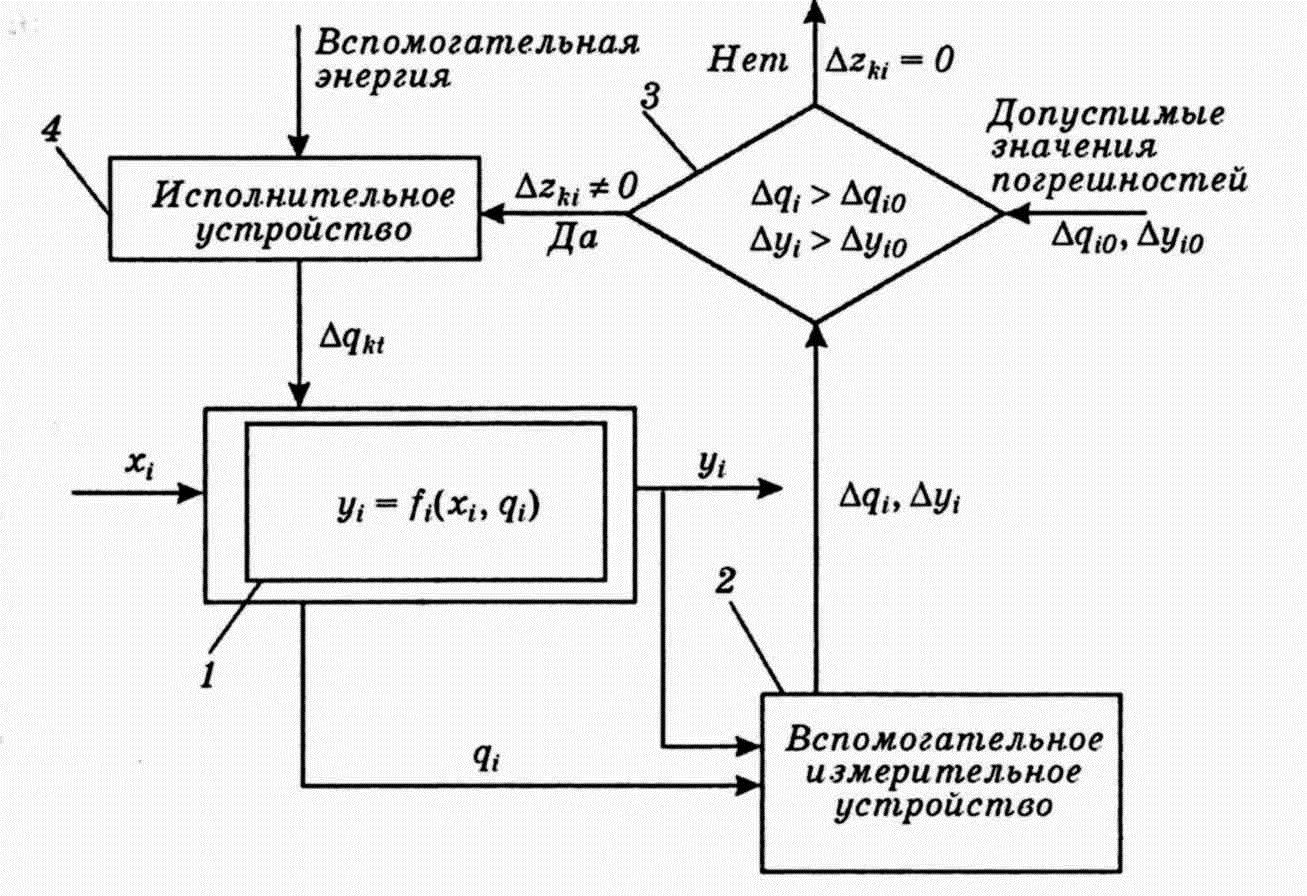
\includegraphics[width=1\textwidth]{11would.png}
	\caption[Юстировка по схеме вспомогательных измерений]{ Юстировка по схеме вспомогательных измерений: 1~-- ОЭП; 3~-- система сравнения погрешностей с их допустимыми значениями; $ x,\,y $ -- информативные параметры входного и выходного сигналов; $ q $~-- конструктивные параметры прибора; $ f $~-- функция, связывающая $ x $ и $ y $; $ y_0, q_0 $ -- расчетные (номинальные) значения перечисленных параметров; $ \Delta z_k $~-- управляющий сигнал на исполнительное устройство; $ \Delta q_k $~-- коррекция исполнительного устройства, изменяющая параметры прибора }
	\label{pic:11would}
\end{figure}

Исполнительное (юстировочное) устройство (инструмент, приспособление, привод) при необходимости с привлечением вспомогательной энергии воздействует на параметры или свойства структурных элементов либо компенсаторов в целях устранения самой погрешности или ее влияния на качество.

По этой схеме происходит юстировка элементов прибора при поузловой сборке и отдельных показателей его качества (регулировка фокусных расстояний объективов, их фокусировка, устранение наклона или биения изображения в зеркально-призменных системах, доводка направляющих поступательного и вращательного движения). Типичным примером является юстировка формы отражающей поверхности адаптивного зеркала по измеренным значениям погрешностей расположения составляющих элементарных зеркал (рис.~\ref{pic:11adapt}).

Коллинеарность и компланарность элементарных зеркал (рис.~\ref{pic:11adapt}) обеспечиваются их совместной полировкой после приклеивания (с последующим нанесением зеркального покрытия) и контроля с помощью пробного стекла или интерферометра либо параллельность~-- с помощью юстировочных винтов~4 и контролем по автоколлиматору, а расположение в одной плоскости~--- подачей посредством электрода~5 напряжения смещения на пьезокерамику, изменяющего размер (высоту) цилиндра с контролем по пробному стеклу или интерферометру.
\ref{pic:11adapt}

\begin{figure}[h!]
	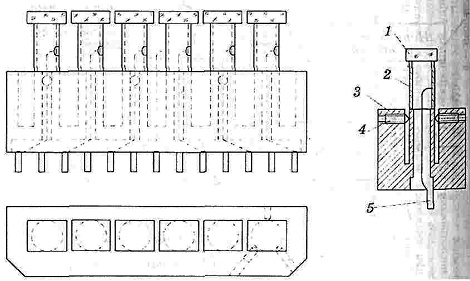
\includegraphics[width=1\textwidth]{11adapt.png}
	\caption[Адаптивное зеркало]{ Адаптивное зеркало: 1 -- отдельное элементарное зеркало; 2 -- цилиндр из пьезокерамики; 3 -- основание; 4 -- юстировочный винт; 5 -- электрод }
	\label{pic:11adapt}
\end{figure}

Способ юстировки по схеме вспомогательных измерений имеет следующие особенностями:
\begin{enumerate}
\item юстируется не суммарный показатель качества прибора, а только его составляющие, обусловленные отличием некоторых первичных, частичных или комплексных погрешностей от их номинального значения;
\item для измерения отклонения каждой погрешности от ее номинального значения необходимо иметь соответствующее вспомогательное измерительное устройство (ВИУ);
\item система сравнения должна содержать для компенсируемых погрешностей их допустимые значения;
\item результат юстировки в существенной степени зависит от качества ВИУ и оптимальной последовательности операций.
\end{enumerate}

\newthought{Юстировка по схеме образцовых сигналов }\marginnote{\allcaps{ЮСТИРОВКА ПО СХЕМЕ ОБРАЗЦОВЫХ СИГНАЛОВ}} основана на том, что на вход прибора (функционального устройства) подается образцовый сигнал $ x_0 $, либо входной сигнал подается также на образцовый прибор (рис.~\ref{pic:11etalon}).

\begin{figure}[h!]
	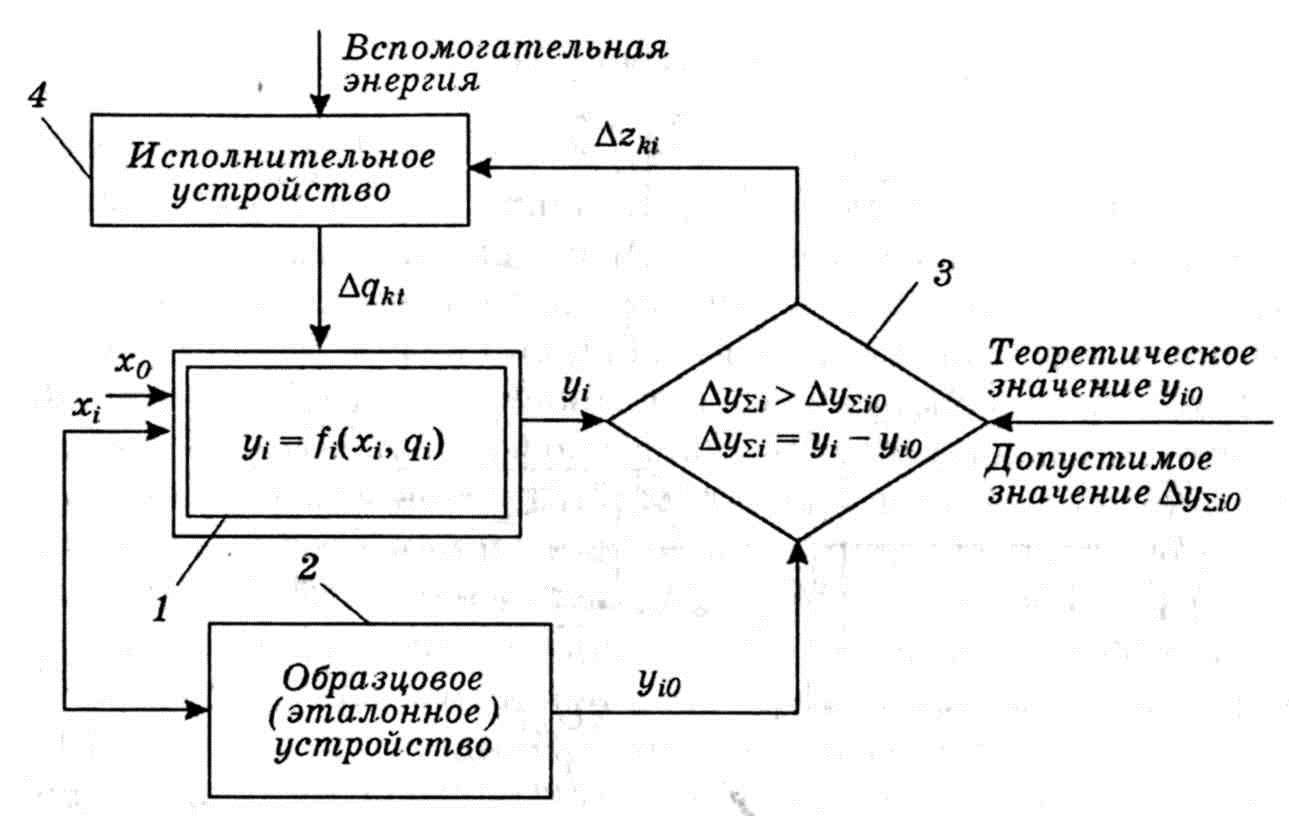
\includegraphics[width=1\textwidth]{11etalon.png}
	\caption[Юстировка по схеме образцовых сигналов]{ Юстировка по схеме\breakобразцовых сигналов }
	\label{pic:11etalon}
\end{figure}

Образцовый сигнал позволяет получить теоретическое (номинальное) значение $ y_{i0} $ информативного сигнала путем расчета по номинальной функции прибора, а образцовый прибор или устройство --- номинальным преобразованием сигнала.

Номинальное значение поступает в систему сравнения, где вычисляется разность значения $ y_{i0} $ и действительного его значения $ y_i $, поступившего с выхода прибора:
\[ \Delta y_{\Sigma i} = y_i - y_{i0} \]

Система сравнения на основании сравнения $ \Delta y_{\Sigma i} $, с его допустимым значением $ \Delta y_{\Sigma i0} $ вырабатывает при $ \Delta y_{\Sigma i} > \Delta y_{\Sigma i0} $ управляющий сигнал $ \Delta z_{ki} $ на исполнительное устройство.

В качестве образцового сигнала используются, например, волновой фронт эталонного источника светового излучения, эталоны угловых и линейных величин (шкалы, призмы, коллиматоры), углы и расстояния между предметами, звездами, длина волн спектральных линий. Образцовыми преобразователями могут быть образцовые (эталонные) приборы, датчики, объективы.

По этой схеме обычно производится окончательная юстировка прибора или его функциональных устройств. 

Юстировка по схеме образцовых сигналов обладает следующими особенностями:
\begin{itemize}
	\item юстируется показатель качества (суммарная погрешность) прибора или устройства, обусловленный влиянием всех действующих на него погрешностей;
	\item необходим образцовый сигнал $ x_0 $,  либо образцовый прибор (устройство), позволяющие получить номинальное значение выходного сигнала $ y_{i0} $; 
	\item юстировка производится в дискретных точках диапазона работы прибора, соответствующих значениям образцового сигнала (например, для определенной длины волны света, конкретного значения угла, дистанции), либо в моментах сравнения показаний юстируемого и эталонного приборов (устройств);
	\item результат юстировки в существенной степени зависит от качества образцового сигнала или эталонного прибора.
\end{itemize}

\section{Юстировочные расчеты}

Юстировка является весьма трудоемким процессом. Она выполняется высококвалифицированными специалистами, требует использования специальной оснастки, инструмента, прецизионных средств контроля. Поэтому к ней следует прибегать только в случае, когда она действительно необходима для достижения требуемых показателей качества либо когда доказана ее экономическая эффективность благодаря расширению допусков на погрешности изготовления деталей, что обычно бывает при единичном и мелкосерийном производствах.

Юстировка прибора и его узлов должна предусматриваться на этапе их проектирования, а не тогда (как это случается), когда прибор изготовлен и юстировку трудно, а иногда и невозможно выполнить. Поэтому на соответствующем этапе проектирования выполняют расчеты, доказывающие необходимость юстировки для получения того или иного показателя качества, устанавливают требования к результатам юстировки (точность юстировки), а также диапазон и чувствительность воздействия на структурные элементы конструкции (диапазон и чувствительность регулировки), которые определяют требования к исполнительному устройству.

От правильного определения необходимого числа юстируемых параметров, требований к точности юстировки, диапазону и чувствительности регулировок, рациональной методики выполнения зависит эффективность юстировки прибора.

Число юстируемых параметров, требования к диапазону и чувствительности их регулировки, методика выполнения юстировки зависят от количества, вида и степени влияния первичных погрешностей, а также от заданных значений показателей качества на проектируемый прибор. Юстировочные расчеты поэтому представляют собой сложную, многофакторную задачу, решение которой должно основываться на моделях, учитывающих взаимосвязь этих факторов.
При этом учитывают значение и характер влияния погрешности (случайное, неслучайное, аддитивное, мультипликативное, периодическое, степенное), условия производства (серийность, наличие необходимого оборудования, квалификацию специалистов) и особенности эксплуатации прибора. 

Эти факторы позволяют выбрать метод компенсации и определить требования к его точности, диапазону и чувствительности регулировок.
Естественно, что вначале выбирают способ устранения или компенсации наиболее сильно влияющей погрешности, а также такой, который позволяет компенсировать не одну, а несколько погрешностей сразу.

Весьма часто не требуется проводить тщательных расчетов для доказательства необходимой юстировки того или иного частного показателя качества, так как априори известно, что его невозможно достичь. В этом случае определяют требования к чувствительности и диапазону юстировки, разрабатывают оптимальную методику ее выполнения.

Методы юстировки типовых ОЭП и функциональных устройств изложены в ряде учебных пособий и публикаций. Следует однако заметить, что методики юстировки современных приборов и функциональных устройств обычно держатся фирмами-производителями этой техники в секрете.
Так как возможность юстировки изделий закладывается на этапе их конструирования, то далее рассмотрим юстировку некоторых типовых функциональных устройств ОЭП.

\section{Юстировка линзовых систем ОЭП}

К линзовым системам ОЭП относятся объективы, окуляры, оборачивающие системы и осветительные устройства. Они предназначены для силового преобразования пучка лучей в целях построения изображения, наблюдения, трансформации, а также освещения предмета наблюдения.

К этим системам предъявляются определенные требования по качеству создаваемого изображения, его расположению относительно других элементов оптической системы, расположению самих линзовых систем относительно предмета наблюдения или изображения и источников освещения.

Обеспечить указанные требования технологически, т.е. только за счет соответствующих допусков на изготовление и сборку элементов линзовых систем, как правило, не удается. Поэтому при разработке их конструкции следует предусматривать (при необходимости) обеспечение указанных требований с помощью юстировки.

Типовыми юстировочными операциями линзовых систем являются:
\begin{itemize}
\item юстировка качества изображения;
\item фокусировка изображения, обеспечение рабочих расстояний;
\item регулировка фокусных расстояний;
\item выставка визирных линий и оптических осей;
\item юстировка увеличения и масштаба изображения.
\end{itemize}

Методы и способы юстировки ОЭП обычно изучаются в специальных курсах учебных дисциплин и изложены в ряде учебных пособий и публикаций. Однако, в связи с тем что юстировка изделий закладывается на этапе конструирования, а линзовые системы являются одними из наиболее распространенных компонентов оптических систем приборов, представляется целесообразным рассмотреть вкратце типовые конструктивные и технологические решения и приемы, позволяющие выполнять перечисленные выше юстировочные операции.

Погрешности\marginnote{\allcaps{ЮСТИРОВКА\break КАЧЕСТВА\break ИЗОБРАЖЕНИЯ}} изготовления и сборки деталей линзовых систем, отклонения характеристик их материалов приводят к возникновению дополнительных аберраций и ухудшают качество создаваемого изображения. Улучшить качество изображения можно компенсацией тех или иных аберраций, превосходящих допустимое значение, соответствующими юстировочными операциями.

Рассмотрим типовые юстировочные операции на примере юстировки качества изображения объективов.

На первом этапе выявляются дефекты качества изображения, создаваемого собранным объективом. 
На практике дефекты из-за технологических погрешностей изготовления и сборки элементов (деталей) объектива обычно выявляют по виду дифракционного изображения точки. 
Объектив устанавливается в параллельном ходе лучей, создаваемом коллиматором~1 от точечной диафрагмы, а дифракционное изображение точки рассматривается с помощью микроскопа 5 визуально или через видеонасадку (рис.~\ref{pic:11control}~а).

Если в дифракционном изображении точки видно яркое неокрашенное светлое пятно, окруженное одним-двумя концентрическими кольцами, не имеющими разрывов и утолщений (идеальное изображение -- рис.~\ref{pic:11control}~б), то объектив изготовлен правильно.

\begin{figure*}[h!]
	\caption[Контроль и устранение дефектов качества изображения]{ Контроль и устранение\breakдефектов качества изображения }
	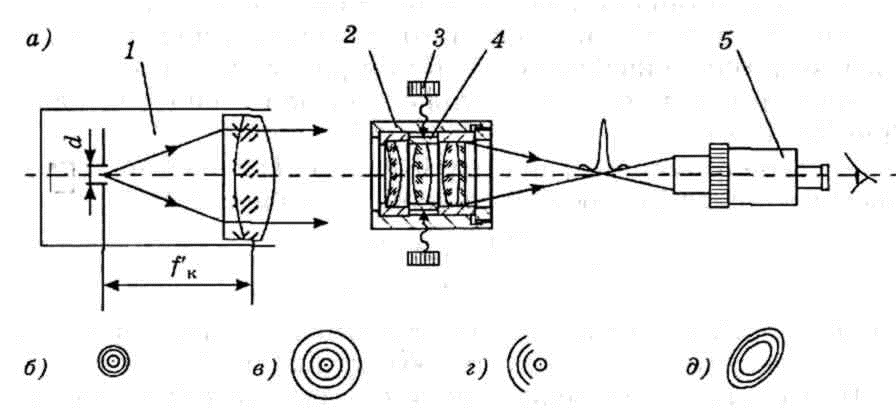
\includegraphics[width=1\textwidth]{11control.png}
	\label{pic:11control}
\end{figure*}

Угловой размер диафрагмы не должен превышать теоретической разрешающей способности объектива:
\[ d \leq \dfrac{120''f_k\,5*10^{-6}}{D_\text{вх}} \]
где $ f_k $ -- фокусное расстояние объектива коллиматора, мм; $ D_\text{вх} $ -- диаметр входного зрачка объектива, мм.

Необходимое увеличение микроскопа находится из условия, что угловой размер радиуса первого дифракционного кружка Эйри должен составлять в пространстве изображений угловое значение, не меньшее, чем разрешающая способность глаза $ \varepsilon $ наблюдателя (принимается для микроскопов равной $ 2'-4' $):
\[ \Gamma = \dfrac{250 \, \varepsilon\, 3*10^{-4}}{1,22 \lambda (f'/D_\text{вх})} = (450\div900) A \]
где  $ \lambda = 0,55 $ мкм -- длина волны света; А -- относительное отверстие контролируемого объектива.

Если используется видеонасадка с ПЗС-матрицей (или микрообъектив проецирует изображение дифракционной точки на ПЗС-матрицу), то необходимое увеличение рассчитывается исходя из характеристик разрешающей способности матрицы.

Увеличение числа колец вокруг ядра (рис.~\ref{pic:11control}~в) указывает на наличие \textit{сферической аберрации}, обусловленной погрешностями изготовления толщины линз и воздушных промежутков, общими погрешностями формы $ N $, погрешностью показателя преломления материалов $ \Delta n_e $, а иногда и ошибкой установки стороны линзы (при близких значениях их радиусов кривизны).

Устранение сферической аберрации производят изменением воздушного промежутка между определенными компонентами (линзами) объектива. Для этого в конструкции либо предусматривают сменное прокладное кольцо между соответствующими линзами или специальное регулировочное кольцо либо подрезают одну из оправ соответствующей линзы.

Если в изображении точки наблюдаются асимметрия в распределении освещенности колец, односторонний их разрыв или несимметричная фигура, называемая \textit{комой} (рис.~\ref{pic:11control}~г), то это говорит о децентрировке компонентов объектива. Она возникает из-за децентрировки линз при изготовлении, из-за смещения в зазорах посадок и наклонов линз, вследствие сдвигов и клиновидности слоя клея при их склеивании, из-за несоосности посадочных гнезд компонентов в оправах и в корпусной детали.

Часть погрешностей, вызывающих децентрировку линзы (или компонента), может быть компенсирована результативной обработкой оправы от ее оптической оси после закрепления линзы.

Однако остаточные децентрировки линз (компонентов) относительно базовых осей оправ, смещения и наклоны самих оправ в корпусе зачастую не обеспечивают необходимой центрировки компонентов оптической системы. В этом случае применяют конструктивные методы компенсации децентрировки сдвигом, разворотом или наклоном одной или нескольких линз объектива.

Сдвиг линзы перпендикулярно к оптической оси осуществляют обычно с помощью технологических винтов~3 (рис.~\ref{pic:11control}~а), смещающих оправу~4 с линзой в пределах зазора между оправой и корпусом~2. Этим смещением создается аберрация противоположного знака по отношению к суммарной аберрации других компонентов, вызванных их децентрировкой. После выполнения юстировки положение линзы, как правило, фиксируется герметиком.

В связи с тем что децентрировки линз представляют собой векторные величины, разворачивая линзу или несколько линз оптической системы объектива вокруг базовой оси оправы, можно компенсировать влияние их децентрировок на качество изображения. Этот прием используют при юстировке объективов теодолитов, фотограмметрических и крупногабаритных объективов.

Наклон линз для компенсации децентрировки используется на практике реже, так как он менее технологичен и применяется обычно для юстировки зеркально-линзовых объективов и крупногабаритных линз.

Изображение точки, вытянутое в одну сторону (рис.~\ref{pic:11control}~д), или крестообразное, переходящее при перефокусировке в горизонтальную либо вертикальную полосы, указывает на астигматизм объектива. Он обусловлен цилиндричностью рабочих (сферических) поверхностей линз, возникающих при их изготовлении или из-за деформации (пережатии) при креплении. Иногда удается устранить этот дефект разворотами компонентов или ослаблением усилий крепления. Чаще всего дефектную линзу (обнаруживаемую при развороте ее оправы вокруг базовой оси) удаляют, заменяя ее бездефектной.

По дифракционному изображению точки можно выявить и устранить и другие технологические погрешности, например грубые свили, <<завалы>> (фаски) по краю линз.

Технологические\marginnote{\allcaps{ФОКУСИРОВКА\break ИЗОБРАЖЕНИЯ}} погрешности изготовления и сборки элементов линзовой системы обычно не позволяют обеспечить необходимое расстояние линзовой системы до объекта наблюдения, других оптических систем или расположение создаваемого изображения в требуемой плоскости.

Возникают такие дефекты, как расфокусировка (нерезкость) изображения, параллакс, погрешность масштаба изображения.

Фокусировка изображения осуществляется продольным (вдоль оптической оси) перемещением линзовой системы, перемещением приемника или других элементов оптической системы прибора.

Необходимая чувствительность перемещения определяется чувствительностью глаза к продольным наводкам, допустимыми значениями параллакса, разномасштабностью или глубиной резкости линзовой системы.

Для определения продольной чувствительности перемещения объектива в целях фокусировки изображения пользуются также приближенными формулами, связывающими его перемещение $ \Delta x $ с перемещением изображения $ \Delta l $ и увеличениями: $ \beta << 1 $ (телескопические),  $ \beta >> 1 $ (микроскопические) и $ \beta = 1 $:
\[ \Delta l \approx \Delta x; \, \Delta l \approx - \beta^2 \Delta x; \, \Delta l \approx \Delta x^2 / f'_\text{об}. \]

Фокусировка линзовых систем при юстировке осуществляется обычно посредством резьбового соединения их оправы с корпусной деталью, с помощью сменных фокусировочных колец (прокладок) либо путем подрезки опорной поверхности.

На рис.~\ref{pic:11objective} изображена конструкция объектива телескопической системы, закрепленного в корпусе~1, с возможностью его фокусировки путем разворота оправы~3, сопряженной с переходной деталью~2 по резьбе. Фиксация отъюстированного положения объектива осуществляется посредством упругой деформации части переходной детали винтом~5.

\begin{figure}[h!]
	\begin{center}
		\caption{ Телескопический объектив в юстируемой оправе }
		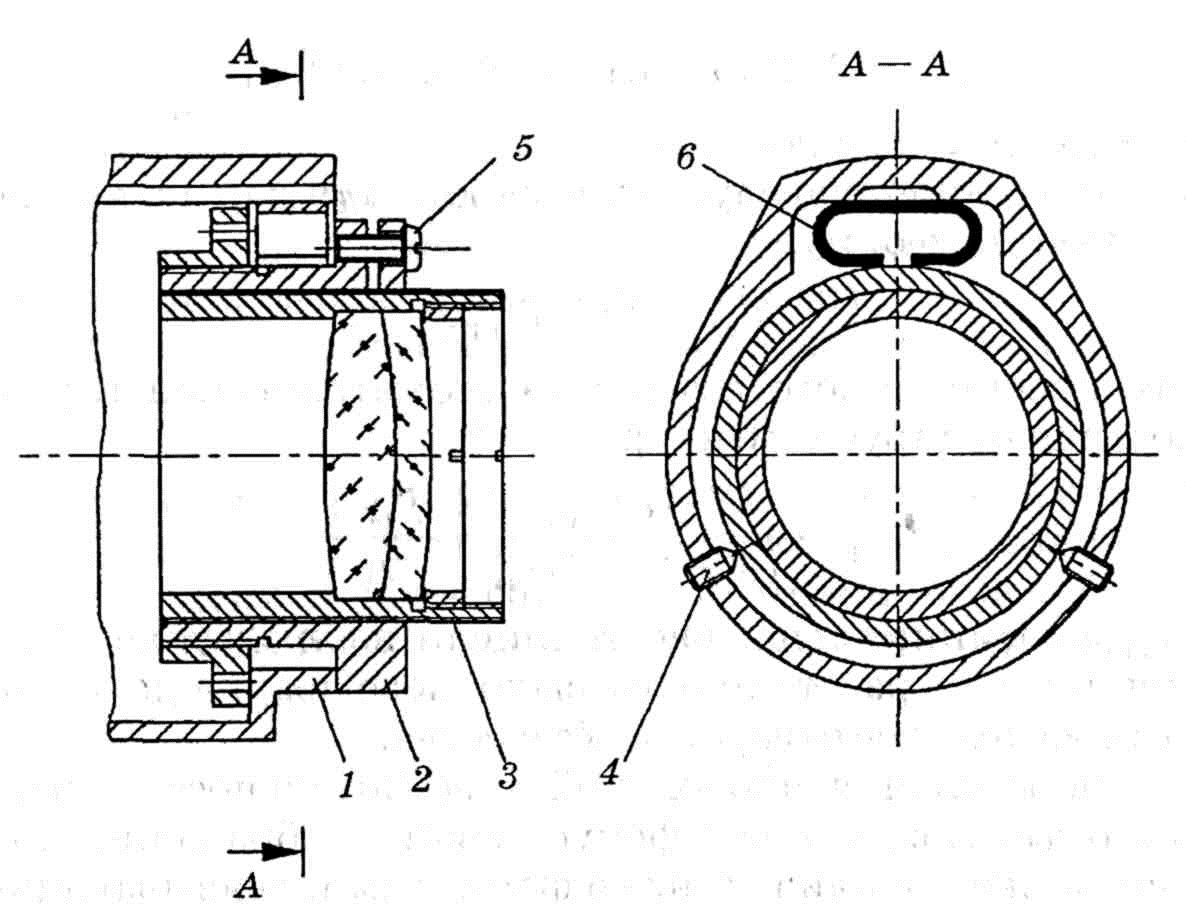
\includegraphics[width=0.8\textwidth]{11objective.png}
		\label{pic:11objective}
	\end{center}
\end{figure}

Для\marginnote{\allcaps{ОБЕСПЕЧЕНИЕ\break РАБОЧИХ\break РАССТОЯНИЙ}} сменных фото- и микрообъективов необходимо обеспечивать с достаточно высокой точностью (до сотых долей миллиметра, иначе появляется недопустимая расфокусировка изображения) расстояние от их опорного торца до плоскости изображения или предметной плоскости, которое называется рабочим расстоянием (высотой).

Рабочее расстояние фотообъектива после его сборки обеспечивается подрезкой опорного торца либо изменением размера специального промежуточного кольца.

Рабочее расстояние (высота) микрообъектива обеспечивается после его сборки подрезкой посадочного торца на специальном станке.

Регулировка фокусных расстояний. Известно, что погрешности фокусных расстояний объективов и окуляров при их серийном производстве достигают значений, равных 0,5-3 \%.

Для ряда измерительных и наблюдательных приборов необходимо, чтобы фокусные расстояния объективов и других линзовых систем отличались от их номинальных значений на существенно меньшее значение, которое не может быть обеспечено при изготовлении.

В тех случаях, когда нецелесообразно или не удается компенсировать влияние погрешностей фокусных расстояний линзовых систем, производят их юстировку изменением расстояния (воздушного промежутка) между компонентами. Необходимый диапазон и чувствительность изменения расстояния $ \Delta d $ между компонентами находят из выражения, связывающего изменение фокусного расстояния системы из двух компонентов с изменением расстояния между компонентами:
\[ \Delta d = \dfrac{\Delta f'_{\Delta d}}{f'^2 \, \Phi_1 \, \Phi_2}, \]
где $ \Delta f'_{\Delta d} $ -- требуемое изменение фокусного расстояния системы линз; $ \Phi_1 \, \Phi_2 $ -- оптические силы юстируемых компонентов; $ f' $ -- фокусное расстояние системы.

На рис.~\ref{pic:11teleobj} изображена конструкция телеобъектива, состоящего из положительного 1 и отрицательного 3 компонентов. Для регулировки его фокусного расстояния отрицательный компонент имеет возможность перемещаться вдоль оси благодаря резьбовому соединению его оправы с корпусом 2.

Фокусное расстояние этого объектива в номинале равно 500~мм, а оптические силы положительного и отрицательного компонентов: $ 1/86,13 $ и $ -1/11,37 $~мм$ ^{-1} $ соответственно. Следовательно, если мы хотим обеспечить регулировку фокусного расстояния объектива с точностью до 0,1 \%, то чувствительность изменения расстояния между компонентами должна быть не ниже значения, определяемого выражением:
\[ \Delta d = \dfrac{0,1f'}{f'^2 \, \Phi_1 \, \Phi_2} \approx 0,002 \text{мм}. \]

\begin{figure}[h!]
	\begin{center}
		\caption{ Телеобъектив }
		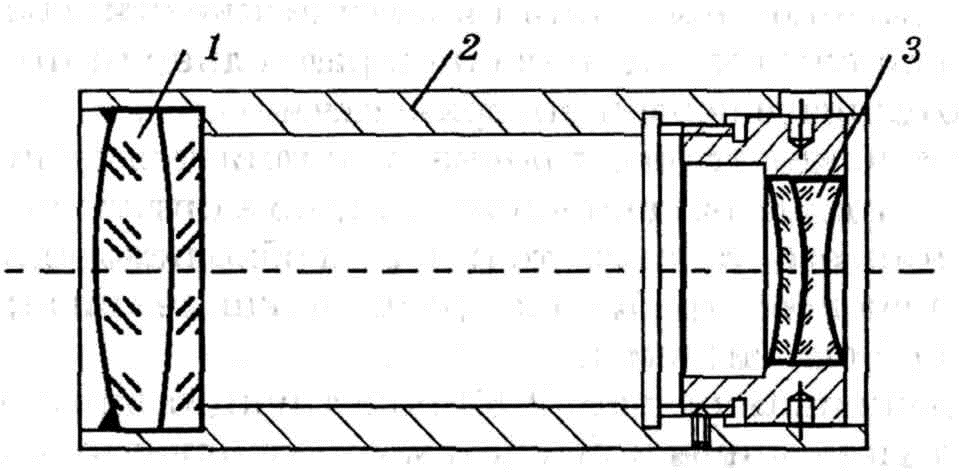
\includegraphics[width=0.75	\textwidth]{11teleobj.png}
		\label{pic:11teleobj}
	\end{center}
\end{figure}

Несмотря на наличие центрировочного пояска на оправе отрицательного компонента, при его вращении трудно обеспечить необходимую точность центрировки компонентов телеобъектива. Поэтому при такой юстировке более предпочтительной считается конструкция, где изменение расстояний между компонентами осуществляется без их разворота. 

В\marginnote{\allcaps{ВЫСТАВКА ВИЗИРНЫХ ЛИНИЙ И ОПТИЧЕСКИХ ОСЕЙ}} ряде приборов, таких как микроскопы, прицелы, автоколлиматоры, бинокулярные приборы, необходимо после их сборки выставлять визирные линии и оптические оси, создаваемые линзовыми системами, соосно, параллельно (или перпендикулярно) другим осям и поверхностям.

Весьма часто эта юстировка выполняется сдвигом всего объектива (окуляра) перпендикулярно к оптической оси для приведения его узловой точки в необходимое положение, обеспечивающее требуемое расположение визирной или оптической оси системы.

Изображенная на рис.~\ref{pic:11objective} конструкция крепления объектива телескопической системы позволяет осуществлять подобную юстировку с помощью винтов~4 и пружины~6.

В\marginnote{\allcaps{ЮСТИРОВКА\breakУВЕЛИЧЕНИЯ И\breakМАСШТАБА\breakИЗОБРАЖЕНИЯ}} предыдущих разделах упоминалось, что при фокусировке линзовой системы или при регулировке ее фокусного расстояния могут изменяться создаваемое увеличение или масштаб изображения. 
В ряде оптических приборов, таких как отсчетные микроскопы, бинокли и бинокулярные микроскопы, профильные проекторы, отсчетные телескопические трубы, двойные дифференциальные отсчетные системы, требуется обеспечивать номинальное увеличение, равенство увеличений в ветвях или номинальную разность увеличений.
Так как эти требования часто не могут быть выполнены с необходимой точностью технологически, то в подобных приборах предусматривается юстировка увеличения или масштаба изображения.

Известно, что линзовая система 1 (объектив), строящая изображение $ y' $ предмета $ y $ (рис.~\ref{pic:11image}), создает масштаб изображения $ M $, равный линейному увеличению объектива $ V $:
\[ M = V = \dfrac{y'}{y} = \dfrac{f'}{z} = \dfrac{S'}{S} =\dfrac{\sin\,\sigma_A}{\sin\,\sigma'_A}, \]
где $ f $ и $ f' $ -- переднее и заднее фокусные расстояния объектива; $ z $ и $ z' $ -- расстояния от переднего фокуса $ F $ до осевой точки предмета и от заднего фокуса $ F' $ до осевой точки изображения, соответственно; $ S $ и $ S' $ -- передний и задний отрезки соответственно; $ \sin\,\sigma_A,\,\sin\,\sigma'_A $ -- апертурные углы в пространстве предметов и изображений соответственно.

Изменением параметров $ z, \, z' ,\, f',\, S,\, S' $ можно юстировать линейное увеличение $ V $ и масштаб изображения $ M $.

\begin{figure}[h!]
	\caption{ Построение изображения предмета линзовой системой }
	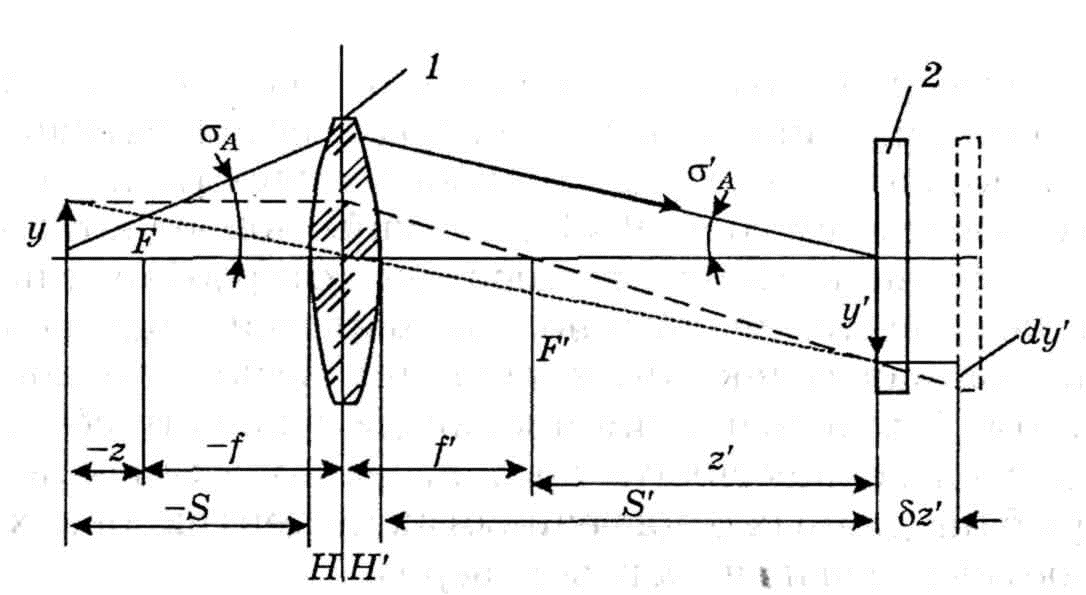
\includegraphics[width=1\textwidth]{11image.png}
	\label{pic:11image}
\end{figure}


\section{Юстировка зеркально-призменных систем}

Зеркально-призменные системы (ЗПС) требуют весьма строгой ориентировки относительно других элементов оптической схемы. Погрешности расположения неподвижных ЗПС в сходящемся ходе лучей приводят к децентрировкам, наклону и перекосу изображения, срезанию поля зрения и зрачков, расфокусировке. Погрешности расположения неподвижных ЗПС в параллельном ходе лучей оказывают меньшее влияние на качество изображения, однако часто требуется их строгая угловая установка относительно некоторых баз прибора.

Погрешность расположения подвижных ЗПС приводит к погрешности функционирования прибора, ухудшению качества изображения и другим дефектам. Рассмотрим кратко влияние погрешностей расположения простейших ЗПС, являющихся эквивалентами большого ряда более сложных ЗПС, на некоторые характеристики качества прибора.

Пусть\marginnote{\allcaps{ЗПС В СХОДЯЩЕМСЯ\breakХОДЕ ЛУЧЕЙ}} плоское зеркало~1 (рис.~\ref{pic:11mirror}) установлено в сходящемся ходе лучей между объективом~2 и матовым экраном или позиционно-чувствительным приемником (например, ПЗС-матрицей)~3, на котором строится изображение. Свяжем с номинальным положением зеркала неподвижную координатную систему $ X,\, Y,\, Z $, а с экраном (приемником)~-- $ X_\text{э},\, Y_\text{э},\, Z_\text{э} $.

\begin{figure}[h!]
	\caption{ Плоское зеркало в\breakсходящемся пучке лучей }
	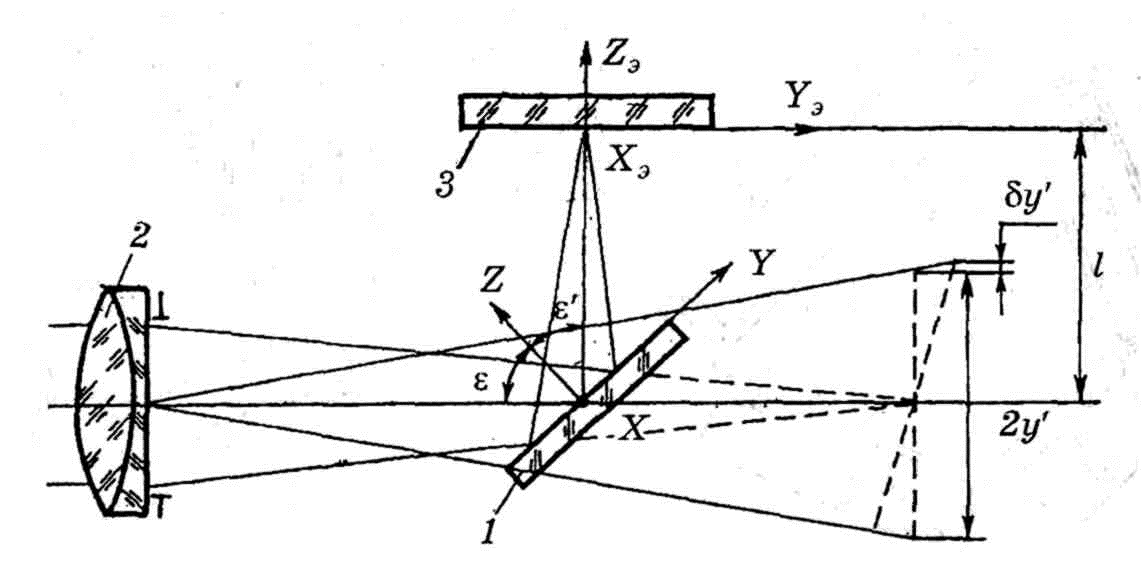
\includegraphics[width=1\textwidth]{11mirror.png}
	\label{pic:11mirror}
\end{figure}

При установке зеркала возможны его линейные и угловые смещения (погрешности) относительно номинального положения. Небольшие смещения зеркала вдоль осей $ Y $ и $ X $ недейственны (так как световой диаметр зеркала обычно выполняется с запасом для устранения срезания светового пучка). Смещение зеркала из номинального положения вдоль оси $ Z $ на величину $ \Delta z $ вызывает параллельный сдвиг отраженного пучка лучей, т.е. сдвиг изображения на экране $ \Delta y_\text{э} $, расфокусировку $ \Delta z_\text{э} $, погрешность размера изображения $ \delta y' $.

Поворот зеркала вокруг оси $ Z $ не опасен. При повороте зеркала вокруг оси $ X $ на угол $ \Delta \varphi_x $ происходят следующие явления:
\begin{itemize}
\item сдвиг изображения по оси $ Y_\text{э} $ -- $ \Delta y_\text{э} $;
\item наклон плоскости изображения относительно оси $ X_\text{э} $ -- $ \Delta \varphi_X $;
\item погрешность размера (масштаба) изображения по оси $ Y $ за счет наклона плоскости изображения -- $ \delta y'_\text{э} $;
\item расфокусировка изображения на оси и на краях~-- $ \Delta z_\text{э.о.} $ и $ \Delta z_\text{э.к.} $.
\end{itemize}

При повороте зеркала вокруг оси $ Y $ на угол $ \Delta \varphi_y $ возникают следующие дефекты:
\begin{itemize}
\item сдвиг изображения по оси $ X_\text{э} $ -- $ \Delta x_\text{э} $;
\item разворот изображения вокруг оси $ Z_\text{э} $ -- $ \Delta \varphi_{Z} $;
\item наклон плоскости изображения (разворот) относительно оси  $ Y_\text{э} $ -- $ \Delta \varphi_Y $;
\item погрешность размера (масштаба) изображения по оси $ X_\text{э} $ -- $ \delta y'_x $;
\item расфокусировка изображения на оси и на краях~-- $ \Delta z_\text{э.о.} $ и $ \Delta z_\text{э.к.} $.
\end{itemize}

Подвижная призма в параллельном пучке лучей. В ряде оптических приборов (панорамические визиры, прицелы, перископы, геодезические инструменты) для исключения поворота изображения, его сканирования, оборачивания используются вращаемые (поворотные) призмы прямого видения типа Дове, призмы-куба, Пехана, Аббе, Уппендаля (рис.~\ref{pic:11prism}).

\begin{figure}[h!]
	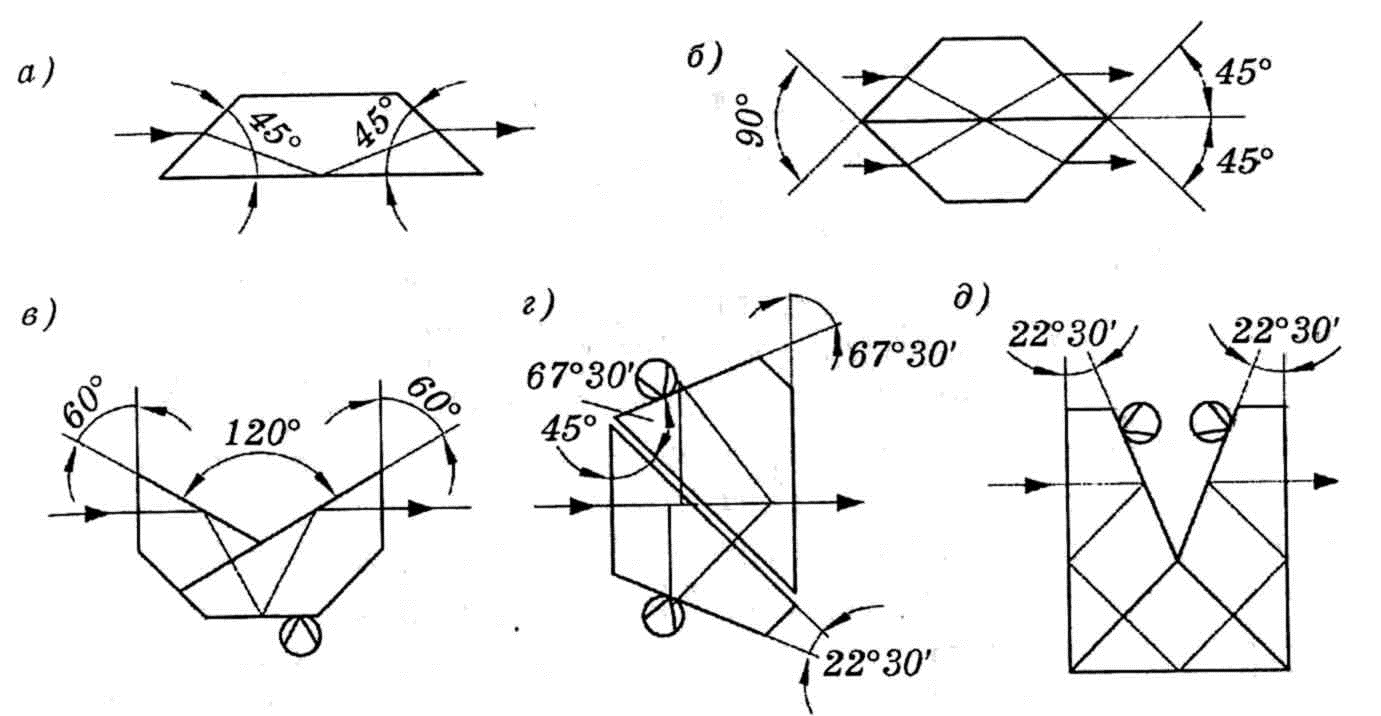
\includegraphics[width=1\textwidth]{11prism.png}
	\caption[Вращаемые (поворотные) призмы прямого видения]{ Вращаемые (поворотные) призмы прямого видения:\breakа -- Дове; б -- куб; в -- Аббе;\breakг -- Пехана; д -- Уппендаля }
	\label{pic:11prism}
\end{figure}

Эти призмы вращаются вокруг оси падающего пучка лучей (визирной оси), вызывая вращение изображения с угловой скоростью в два раза более высокой, чем поворот призмы, и эквивалентны по своему действию плоскому зеркалу и плоско-параллельной пластине или зеркальному ромбу.

Погрешности изготовления и сборки призм приводят к тому, что изображение не только вращается вокруг своей оси, но и претерпевает биение в пространстве. Это биение приводит к погрешности измерения, визирования в приборе и устраняется (уменьшается) путем юстировки узлов призм после их сборки.

Влияние пирамидальности призмы на биение изображения устранить юстировкой нельзя, поэтому при изготовлении призмы назначают «жесткий» допуск на $ \pi $ исходя из условия, что эта погрешность не должна оказывать заметного влияния на биение изображения.

Юстировкой призмы устраняют биение изображения из-за непараллелъности оси вращения призмы к визирной оси коллиматора, и из-за  коллимационной погрешности – погрешности наклона отражающей грани призмы к собственной оси вращения.

Эти\marginnote{\allcaps{УЗЛЫ КРЕПЛЕНИЯ И ЮСТИРОВКА СЕТОК,\breakШКАЛ, РАСТРОВ}} детали крепятся в своих оправах такими же способами, как и другие типовые оптические детали. Если, например, сетка круглая, то она обычно закрепляется в оправе завальцовкой, приклеиванием, резьбовым или накладным кольцом. 
Если деталь не круглая, то она закрепляется прижимными планками, пружинными лапками, приклеиванием.

Измерительные сетки, шкалы, растры, дифракционные решетки являются эталонными элементами функциональных устройств, поэтому при их креплении в оправах и эксплуатации не должно возникать деформаций их рабочих поверхностей. Данное требование обеспечивается при соблюдении таких принципов конструирования соединений, как: статической и геометрической определенностей, силового замыкания, учета тепловых свойств соединяемых деталей.
Главной особенностью конструкций узлов крепления является то, что в них обязательно должна быть предусмотрена юстировка пространственных положений марок, нанесенных на закрепляемые детали относительно их оправ либо вместе с оправами относительно других деталей или баз проектируемых устройств.

Узлы визирных и измерительных сеток необходимо иметь возможность смещать перпендикулярно к оптическим осям и вращать их вокруг них для создания требуемых пространственных расположений визирных осей и плоскостей оптических систем.

Лимбы и круговые растры необходимо центрировать относительно базовых поверхностей их оправ или осей вращения.

Линейные шкалы, растры, измерительные дифракционные решетки необходимо устанавливать параллельно базам оправы или направлениям перемещений.
Спектральные дифракционные решетки, как правило, необходимо разворачивать вокруг всех трех пространственных осей. 
В ряде конструкций решетку устанавливают в оправе на три регулируемые точечные опоры, позволяющие наклонять ее в двух плоскостях относительно базовой поверхности.
Чаще же всего решетка закрепляется в оправе (со строгим соблюдением условия отсутствия ее деформации при креплении и эксплуатации), которая разворачивается относительно базовой корпусной детали узла.
